\documentclass[18pt]{beamer}
\usepackage[utf8]{inputenc} % for the umlauts
\usepackage{subfigure}

\beamertemplatenavigationsymbolsempty
%% SLIDE FORMAT

% use 'beamerthemekit' for standard 4:3 ratio
% for widescreen slides (16:9), use 'beamerthemekitwide'

\usepackage{templates/beamerthemekit}
% \usepackage{templates/beamerthemekitwide}

\setcounter{tocdepth}{1}

%% TITLE PICTURE

% if a custom picture is to be used on the title page, copy it into the 'logos'
% directory, in the line below, replace 'mypicture' with the 
% filename (without extension) and uncomment the following line
% (picture proportions: 63 : 20 for standard, 169 : 40 for wide
% *.eps format if you use latex+dvips+ps2pdf, 
% *.jpg/*.png/*.pdf if you use pdflatex)

%\titleimage{mypicture}

%% TikZ INTEGRATION

% use these packages for PCM symbols and UML classes
% \usepackage{templates/tikzkit}
% \usepackage{templates/tikzuml}

% the presentation starts here

\usepackage{csquotes}
\usepackage{mathabx}
\usepackage{picture}
\usepackage[absolute,overlay]{textpos}
%\usepackage[texcoord,grid,gridunit=mm,gridcolor=red, subgridcolor=green]{eso-pic}
\setbeamercovered{invisible}
\setbeamertemplate{caption}{\raggedright\insertcaption\par}

\title[SWT1]{Softwaretechnik 1 - 4. Tutorium}
\subtitle{Tutorium 17}
\author{Felix Bachmann}
\date{25.06.2019}

\institute{KIT - Institut für Programmstrukturen und Datenorganisation (IPD)}
\begin{document}

% change the following line to "ngerman" for German style date and logos
\selectlanguage{ngerman}

%title page
\begin{frame}
\titlepage
\end{frame}

\section{Evaluation}
	\begin{frame}{Evaluation der Evaluation}
	\centering
		\begin{tabular}{|c|c|}
			\hline 
			Gut & Schlecht/Verbesserungswürdig \\ 
			\hline
			%TODO
			\hline 
		\end{tabular} 
	\end{frame}

\section{Feedback}
	\begin{frame}
	\frametitle{3. Übungsblatt Statistik}
	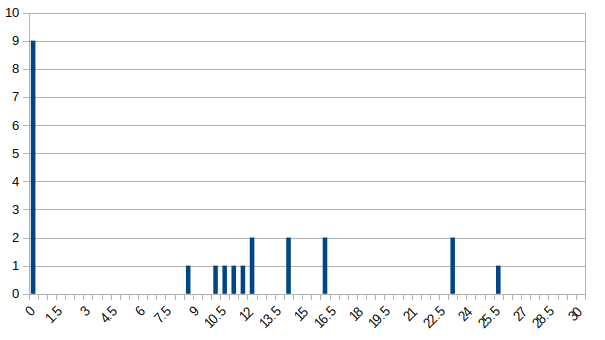
\includegraphics[scale=0.7]{./pics/tut3/statistics-ub3.png}
\end{frame}

\begin{frame}{Häufige Fehler: Blatt 3}
\begin{block}{Programmieraufgaben generell}
	\begin{itemize}
		\item wie letztes Mal gesagt \pause
		\item und das Mal davor \pause
		\item und das Mal davor \pause
		\item und das Mal davor \pause
		\item CheckStyle und Co.
		\pause
		\item nicht am JMJRST-Stil orientieren
		\begin{itemize}
			\item das können wir besser :)
		\end{itemize}
	\end{itemize}
\end{block} 

\begin{block}{Aufgabe 1 (\texttt{PluginManagement} + \texttt{PluginForJMJRST})}
\begin{itemize}
	\pause
	\item Plugins anhand \textbf{Klassen}namen vergleichen, 
	\begin{itemize}
		\item nicht \texttt{Object::getName()}
		\item nicht \texttt{PluginForJMJRST::getName()}
		\item z.B. \texttt{Object::getSimpleName()}
	\end{itemize}
\end{itemize}
\end{block}
\end{frame}

\begin{frame}{Häufige Fehler: Blatt 3}
	\begin{block}{Aufgabe 2 (Instagrim Plug-In)}
	\begin{itemize}
		\pause
		\item Kommentarmenge komisch umgesetzt
		\begin{itemize}
			\item am einfachsten: String-Array
			\item dann aber keine magic numbers verwenden
			\begin{itemize}
				\item z.B. beim Ziehen der zufälligen Kommentare
			\end{itemize}
		\end{itemize}
		\pause
		\item Frame für \texttt{configure()}-Aufruf selbst gebaut
		\begin{itemize}
			\item kein Abzug solange kein Quatsch passiert und sinnvoll programmiert
			\item geht aber auch deutlich einfacher (siehe MuLö)
		\end{itemize}
	\end{itemize}
	\end{block}\pause

	\begin{block}{Aufgabe 3 (iMage-Bundle)}
	\begin{itemize}
	\item keine :D
	\end{itemize}
	\end{block}
\end{frame}

\begin{frame}{Häufige Fehler: Blatt 3}
\begin{block}{Aufgabe 4 (Aktivitätsdiagramm)}
	\begin{itemize}
	\pause 
	\item wie schon bei Anwendungsfalldiagramm
	\begin{itemize}
		\item Aktivitäten enthalten Verben
		\begin{itemize}
			\item es geht darum wer etwas tut
			\item \enquote{Startseite} ist keine Aktivität
			\item \enquote{Startseite anzeigen} schon
		\end{itemize}
	\end{itemize} \pause
	\item keine Partition verwendet/ falsche Syntax \pause
	\item Aktivitiäten = runde Ecken, Objekte = spitze Ecken \pause
	\item $\lbrack$\texttt{Bedingung}$\rbrack$ \pause
	\item Modellierung der Nutzerinteraktion
	\begin{itemize}
		\item z.B. \enquote{Klick} nachdem \enquote{Startseite anzeigen} vorbei? nicht sinnvoll
	\end{itemize}
	\end{itemize}
	\end{block}
\end{frame}

\begin{frame}{Häufige Fehler: Blatt 3}
	\begin{block}{Aufgabe 5 (Zustandsdiagramm)}
		\begin{itemize}
			\pause
			\item Übergänge von innerem parallelen Zustand \texttt{VxW} nach außen (\texttt{A}, \texttt{I})
			\begin{itemize}
				\item \texttt{VxW} ist auch nur ein Zustand
				\item auch wenn \enquote{innen drin} auch noch was passiert
				\item war in MuLö leider auch erst falsch
				\begin{itemize}
					\item deswegen bei einigen Korrekturen evtl. etwas Geschmiere an der Stelle, sorry!
				\end{itemize}
			\end{itemize}
		\end{itemize}
	\end{block}
\end{frame} 

\begin{frame}[fragile]{Häufige Fehler: Blatt 3}
	\begin{block}{Aufgabe 6 (Sequenzdiagramm)}
		\begin{itemize}
			\item allerlei Syntax-Kram
			\begin{itemize}
				\item Lebenslinien, Kästen, Doppelpunkte, Rückgabe-Notation
				\item asynchron vs. synchron (Pfeilspitzen wichtig) 
				\item kein Doppelpunkt bei \enquote{statischen Kästen} 
				\item \texttt{create} zeigt auf Kasten, nicht Lebenslinie/Steuerungsfokus
			\end{itemize}
			\pause
			\item Achtung: Steuerungsfokus ist zwar optional, erhöht aber stark die Lesbarkeit. In Klausur bitte verwenden. Bei Selbstaufrufen sonst problematisch, da Rückgabe ebenfalls optional. \pause
			\item Vorsicht bei Objekt-Zerstörung 
			\begin{itemize}
				\item \texttt{CameraCurve} vor Verwendeung zerstört
			\end{itemize}
		\end{itemize}
	\end{block}
	
\end{frame}

\begin{frame}[fragile]{Häufige Fehler: Blatt 3}
	\begin{block}{Aufgabe 7 (Substitutionsprinzip: Logger)}
		\begin{itemize}
			\pause
			\item Varianz war kein Problem
			\begin{itemize}
				\item getter: Kovarianz bei Rückgabetyp passt
				\item setter: Invarianter Parametertyp passt
			\end{itemize} \pause
			\item Problem war Verhalten, schwächere Nachbedingung \pause
			\item wurde oft zu schwammig formuliert
			\begin{itemize}
				\item oft sowas wie \enquote{Unterklasse tut nicht mehr dasselbe wie Oberklasse}
				\item aber das soll sie ja auch nicht, dann bräuchten wir kein Überschreiben von Methoden :)
			\end{itemize}
			\item bei solchen Aufgaben immer  aus Klient-Sicht anschauen
		\end{itemize}
	\end{block}
\end{frame}

\begin{frame}[fragile]{Häufige Fehler: Blatt 3}
	\begin{columns}
		\begin{column}{0.5\textwidth}
			\begin{verbatim}
			O o = new O();
			o.m(x);
			
			O o = new U(); 
			o.m(x);
			\end{verbatim}
		\end{column}%
		\begin{column}{0.5\textwidth}
			\begin{itemize}
				\item zweiter Aufruf \enquote{muss sich so verhalten wie} erster Aufruf
				\item Vorbedingung schwächer/gleich
				\item Nachbedingung stärker/gleich
			\end{itemize}
		\end{column}
	\end{columns}
	\pause
	\begin{itemize}
		\item \enquote{Unterklasse darf weniger verlangen, muss aber mehr leisten}
		\item (oder gleich viel)
		\item Hintergrund: Klient muss Unterklasse so benutzen können wie Oberklasse. Würde die Unterklasse bspw. mehr verlangen als Oberklasse müsste Klient wissen, dass er Unterklasse benutzt, um sie korrekt aufrufen zu können.
	\end{itemize}
\end{frame}


	\subsection{Feedback 4. Übungsblatt}
	\begin{frame}
		\frametitle{4. Übungsblatt Statistik}
		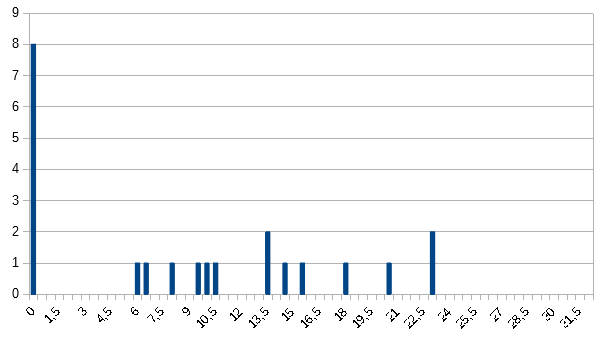
\includegraphics[scale=0.7]{./pics/tut4/statistics-ub4.png}
	\end{frame}
	
	\subsection{4. Übungsblatt - Fehler}
	\begin{frame}
		\frametitle{Häufige Fehler}
		\begin{block}{Aufgabe 1: GUI für iMage}
			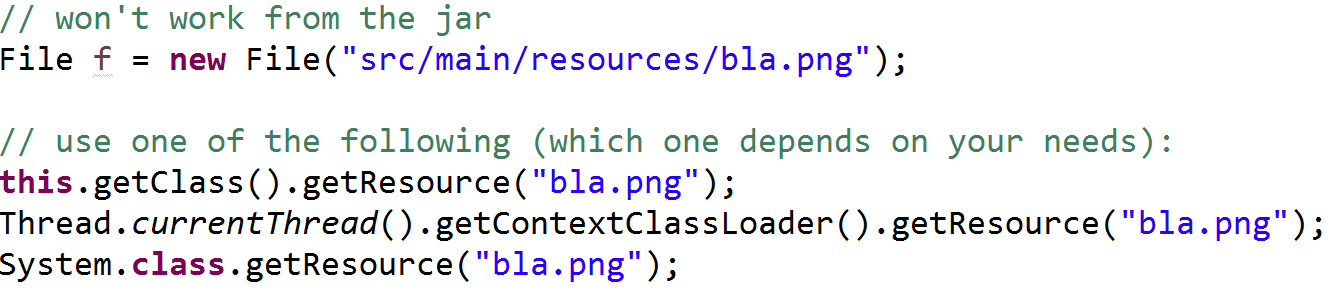
\includegraphics[scale=0.34]{./pics/tut5/file-resource.png}
			\begin{itemize}
				\pause 
				\item Gottklassen, wir wollen aber sinnvolle Objektorientierung! \pause
				\item $\texttt{SwingUtilities.invokeLater(e -> startGui())}$ benutzen:
				\linebreak $\implies$ Thread-Safe (siehe nächstes Tut) \pause
			\end{itemize}
		\end{block}
	\end{frame}

	\begin{frame}
		\frametitle{Häufige Fehler}
		\begin{block}{Aufgabe 2: Zustandsdiagramm für Wasserzeichnen}
			\begin{itemize}
				\item $a() [b] \ne [b] /a()$ \linebreak $\implies$ beim skalieren/exception werfen
				\pause 
				\item sowohl \enquote{validiertes Bild} als auch \enquote{skaliertes Bild} ein Zustand
			\end{itemize}
		\end{block}
		\pause 
		\begin{block}{Aufgabe 3: git}
			\begin{itemize}
				\item bei Umbenennung und Änderung direkt zu commiten würde beides hinzufügen \pause
				\linebreak $\implies$ entweder \texttt{add -N}, \texttt{add -p} \pause
				\linebreak $\implies$ oder \texttt{mv neu alt}, \texttt{git mv alt neu} \pause
				\item git rm -r löscht rekursiv Ordner (inkl. der Überordner!)
				\begin{itemize}
					\item und fügt implizit zur Staging Area hinzu, kein add nötig
				\end{itemize}
			\end{itemize}
		\end{block}
	\end{frame}

	\begin{frame}
		\frametitle{Häufige Fehler}
		\begin{block}{Aufgabe 4: Architekturstile für JMJRST}
			\begin{itemize}
				\item Zuordnung begründen, wenn unklar \pause
				\item Main eindeutig zugeordnet \pause
				\item Änderungen zu vage beschrieben
			\end{itemize}
		\end{block}
	\end{frame}

	\begin{frame}
	\frametitle{Evaluation}
	leider nur 5 Teilnehmer??
	\centering
	\begin{table}
		\begin{tabular}{|c|c|}
			\hline 
			Gut & Schlecht/Verbesserungswürdig \\ 
			\hline
			Folien (3) & \\
			Beispiele und Code (3) & \\ 
			Erklärungen (2) & \\
			Tipps (2) & \\
			Aufgaben (2)&  zu viel Zeit für Aufgaben (2)\\ 
			&  Wahr/Falsch zu einfach (1)\\ 
			& nicht immer Lösungen auf Folie (1)\\
			& gleiche Beispiele wie in VL (1) \\
			& Bewertungen zu kurz (1)\\
			\hline 
		\end{tabular} 
	\end{table}

	\end{frame}

\section{Recap}
	\subsection{Quiz(Adapter)}
	\begin{frame}
		\frametitle{Was bisher geschah..}
		\begin{itemize}
			\item haben uns Entkopplungmuster angeschaut \pause
			\linebreak $\implies$ Beobachter, Iterator, Adapter, Stellvertreter \pause
		\end{itemize}
		\begin{figure}
			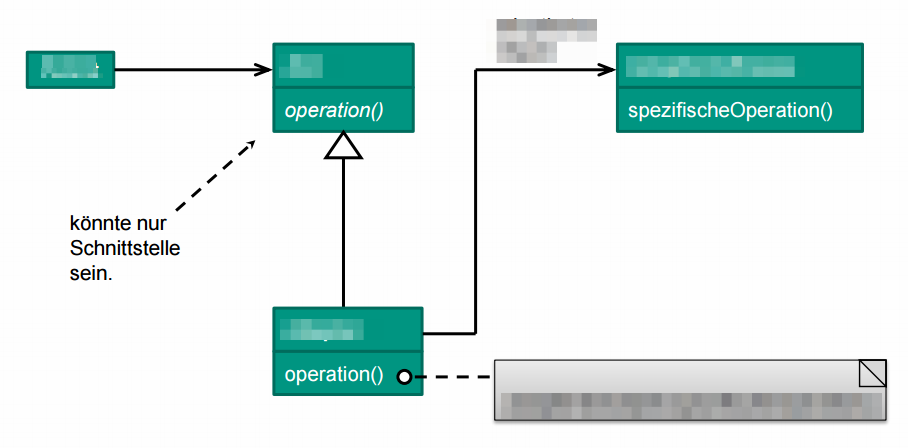
\includegraphics[scale=0.33]{./pics/tut4/adap-obj-mod.png}
		\end{figure}
		Welches Entwurfsmuster? \pause (Objekt-)Adapter
	\end{frame}
	
	\begin{frame}
		\frametitle{Was bisher geschah..}
		\begin{itemize}
			\item haben uns Entkopplungmuster angeschaut
			\linebreak $\implies$ Beobachter, Iterator, Adapter, Stellvertreter
		\end{itemize}
		\begin{figure}
			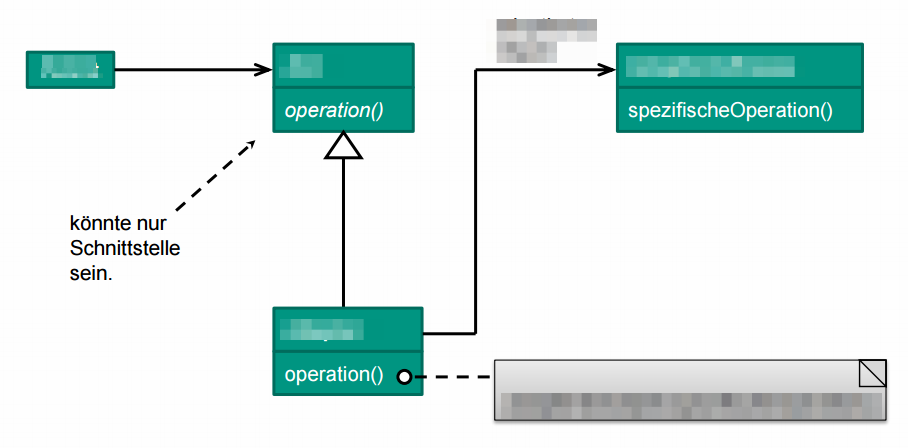
\includegraphics[scale=0.33]{./pics/tut4/adap-obj-mod.png}
		\end{figure}
		Welche Klassen?
	\end{frame}
	
	\begin{frame}
		\frametitle{Was bisher geschah..}
		\begin{itemize}
			\item haben uns Entkopplungmuster angeschaut
			\linebreak $\implies$ Beobachter, Iterator, Adapter, Stellvertreter
		\end{itemize}
		\begin{figure}
			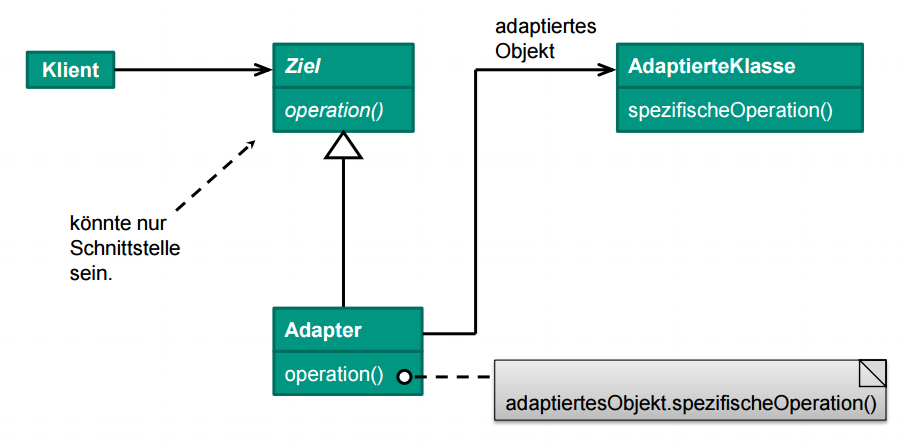
\includegraphics[scale=0.45]{./pics/tut3/adap-obj.png}
		\end{figure}
	\end{frame}
	
	\subsection{Quiz (Iterator)}
	\begin{frame}
		\frametitle{Was bisher geschah..}
		\begin{itemize}
			\item haben uns Entkopplungmuster angeschaut
			\linebreak $\implies$ Beobachter, Iterator, Adapter, Stellvertreter
		\end{itemize}
		\begin{figure}
			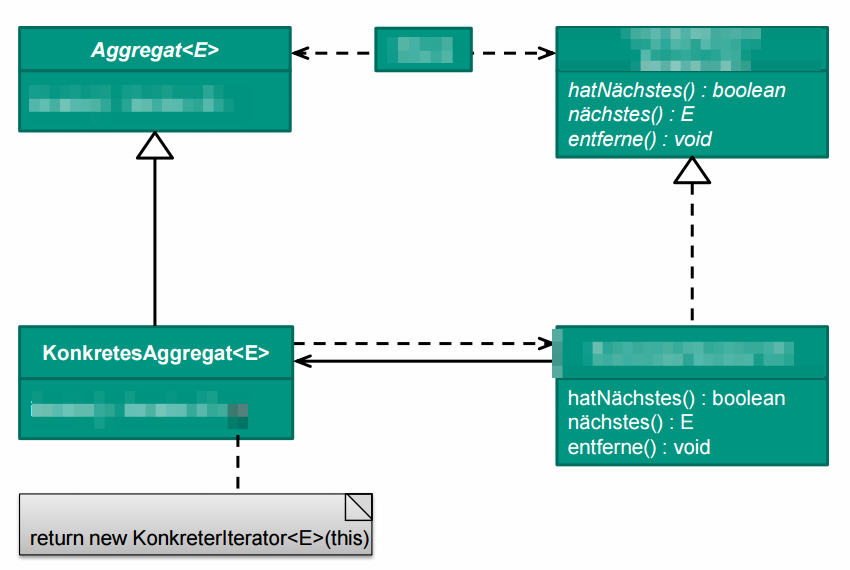
\includegraphics[scale=0.25]{./pics/tut4/iter-mod.png}
		\end{figure}
		Welches Entwurfsmuster? \pause Iterator
	\end{frame}
	
	\begin{frame}
		\frametitle{Was bisher geschah..}
		\begin{itemize}
			\item haben uns Entkopplungmuster angeschaut
			\linebreak $\implies$ Beobachter, Iterator, Adapter, Stellvertreter
		\end{itemize}
		\begin{figure}
			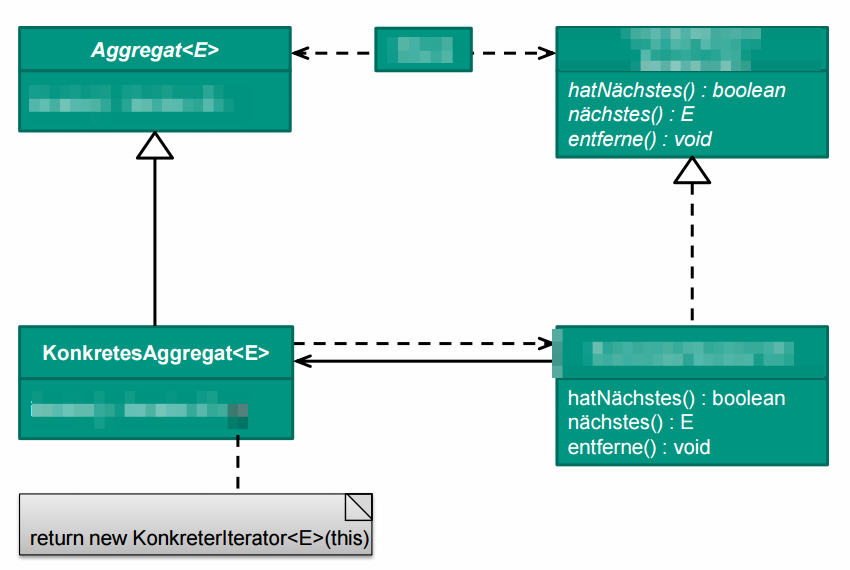
\includegraphics[scale=0.25]{./pics/tut4/iter-mod.png}
		\end{figure}
		Welche Klassen und Methoden?
	\end{frame}
	
	\begin{frame}
		\frametitle{Was bisher geschah..}
		\begin{itemize}
			\item haben uns Entkopplungmuster angeschaut
			\linebreak $\implies$ Beobachter, Iterator, Adapter, Stellvertreter
		\end{itemize}
		\begin{figure}
			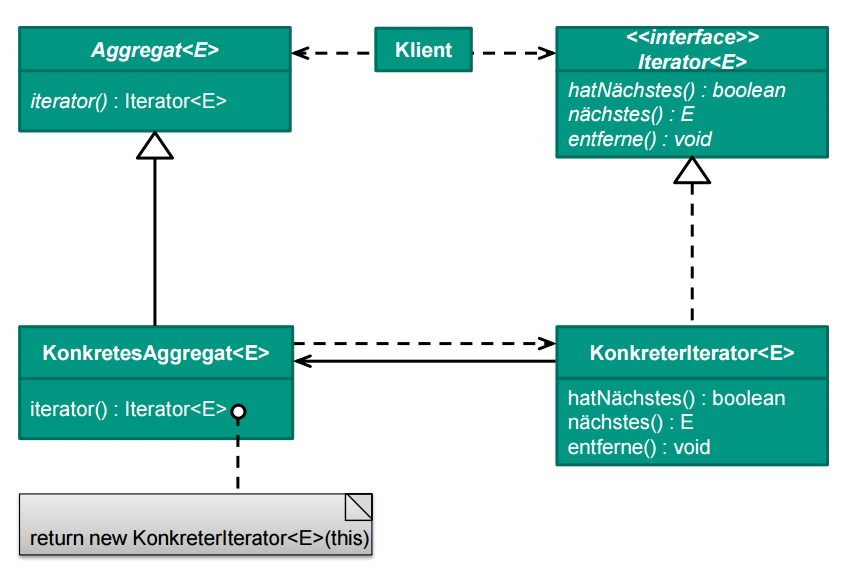
\includegraphics[scale=0.35]{./pics/tut3/iter.png}
		\end{figure}
	\end{frame}
	
	\subsection{Quiz(Beobachter)}
	
	\begin{frame}
		\frametitle{Was bisher geschah..}
		\begin{itemize}
			\item haben uns Entkopplungmuster angeschaut
			\linebreak $\implies$ Beobachter, Iterator, Adapter, Stellvertreter
		\end{itemize}
		\begin{figure}
			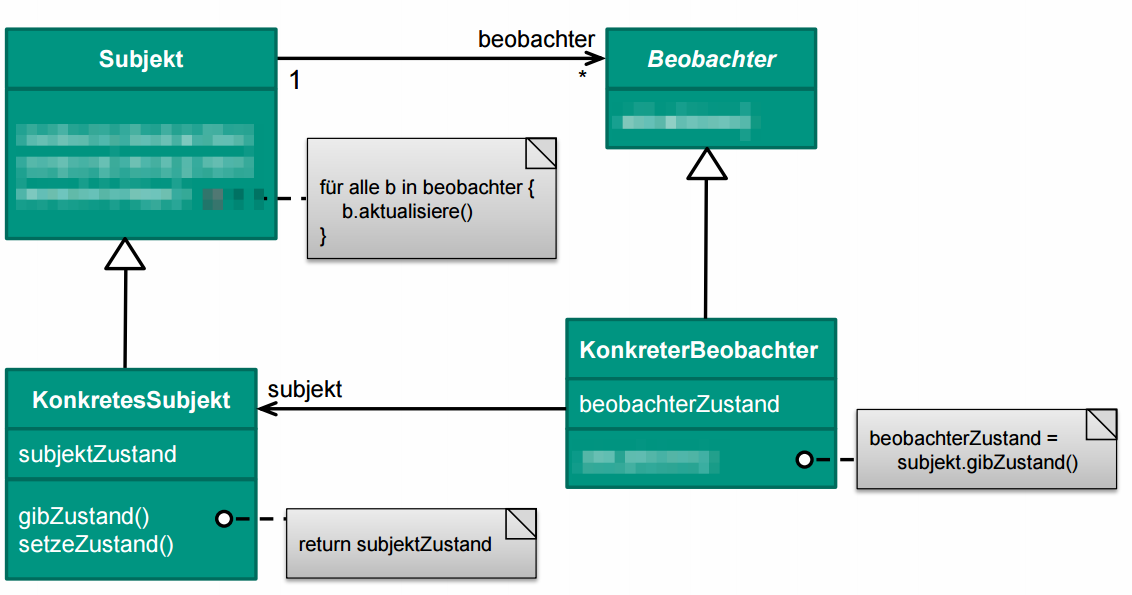
\includegraphics[scale=0.25]{./pics/tut4/obs-mod.png}
		\end{figure}
		\pause Ist wohl ein Beobachter :) \pause Methoden?
	\end{frame}
	
	\begin{frame}
		\frametitle{Was bisher geschah..}
		\begin{itemize}
			\item haben uns Entkopplungmuster angeschaut
			\linebreak $\implies$ Beobachter, Iterator, Adapter, Stellvertreter
		\end{itemize}
		\begin{figure}
			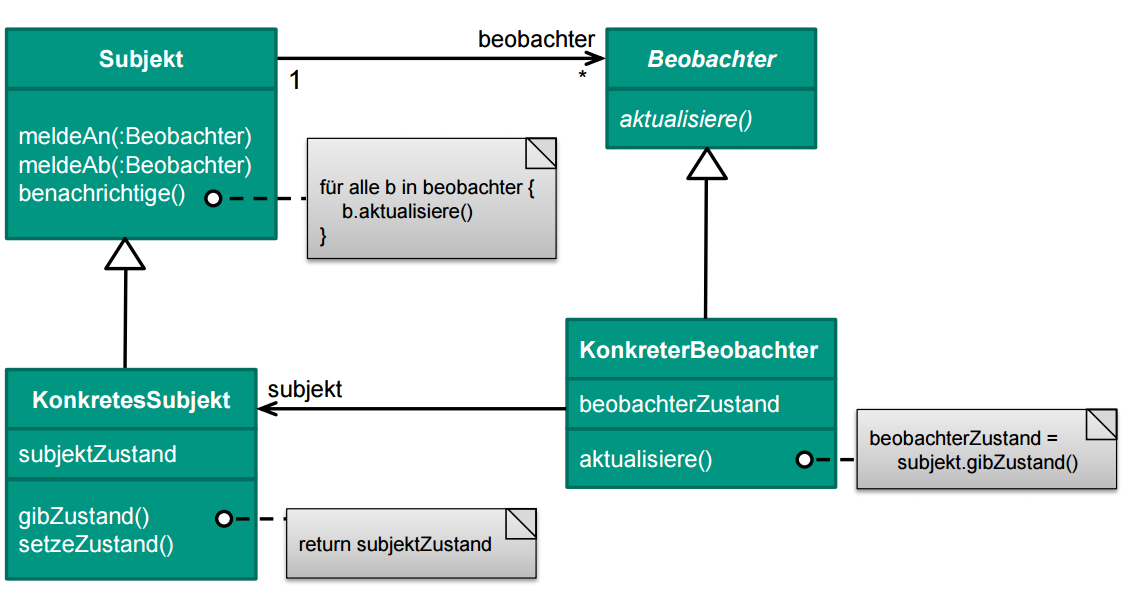
\includegraphics[scale=0.35]{./pics/tut3/obs.png}
		\end{figure}
	\end{frame}

\section{Vermittler}
\subsection{Letztes Entkopplungsmuster: Vermittler}
	\begin{frame}
	\frametitle{Vermittler}
	\begin{block}{Problem}
		\begin{itemize}
			\item mehrere voneinander abhängige Objekte \linebreak \pause $\implies$ Zustände der Objekte von anderen Zuständen abhängig
		\end{itemize}
	\end{block}
	\pause
	\centering
	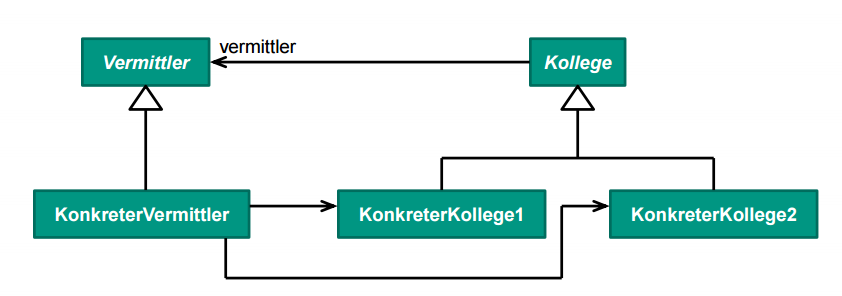
\includegraphics[scale=0.45]{./pics/tut3/med.png}
\end{frame}

\begin{frame}
	\frametitle{Vermittler}
	\centering
	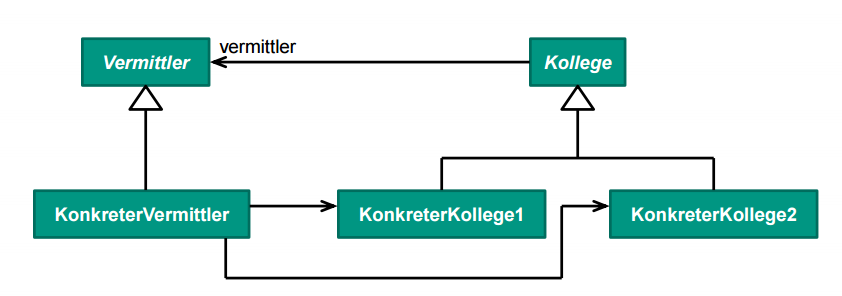
\includegraphics[scale=0.45]{./pics/tut3/med.png}
	\begin{block}{Entkopplung?}
	\begin{itemize}
		\pause 
		\item Kollegen kennen sich nicht direkt  \linebreak \pause $\implies$ Hinzufügen eines Kollegen erfordert keine Änderung der alten Kollegen
	\end{itemize}
	\end{block}
\end{frame}

\begin{frame}{Beobachter vs. Vermittler}
	\begin{itemize}
	\item wirken ähnlich
	\begin{itemize}
	\item ein Vermittler, viele Kollegen
	\item ein Subjekt, viele Beobachter
	\end{itemize}
	\end{itemize}
	\pause
	\begin{block}{Beobachter}
	Beobachter interessieren sich nicht füreinander. Nur für das Subjekt
	\end{block}
	\begin{block}{Vermittler}
	Kollegen interessieren sich füreinander, kommunizieren über den Vermittler miteinander.
	\end{block}
\end{frame}

\subsection{Aufgabe}
	\begin{frame}
	\frametitle{Klausuraufgabe (Hauptklausur SS 2012)}
	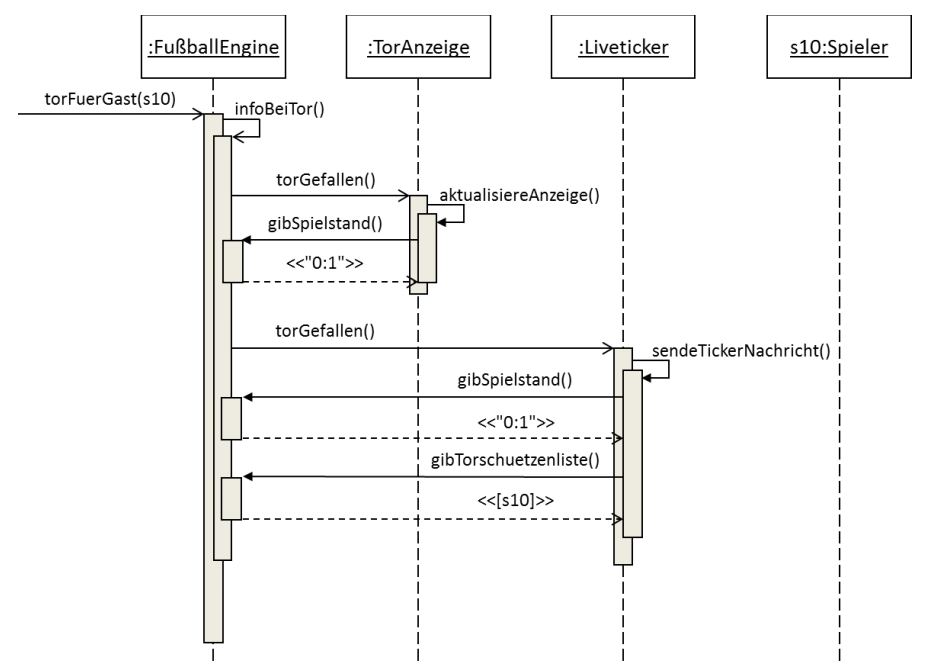
\includegraphics[scale=0.35]{./pics/tut3/obs-task.png}	
	\begin{block}{Aufgabe 1}
	Welches Entwurfsmuster erkennen Sie in diesem Diagramm? \pause
	Beobachter.
	\end{block}
\end{frame}

\begin{frame}
	\begin{small}
	Entwerfen Sie das folgende Klassendiagramm passend zu dem Sequenzdiagramm; es soll
	alle verwendeten Klassen und Methoden enthalten. Kennzeichnen Sie die Zugreifbarkeiten
	der Methoden mit den Symbolen +, -, \#; seien Sie dabei möglichst restriktiv. Verzichten
	Sie auf die Modellierung von Attributen. Kennzeichnen Sie die Elemente
	des Entwurfsmusters und deren Funktion.
	\end{small}
	\linebreak
	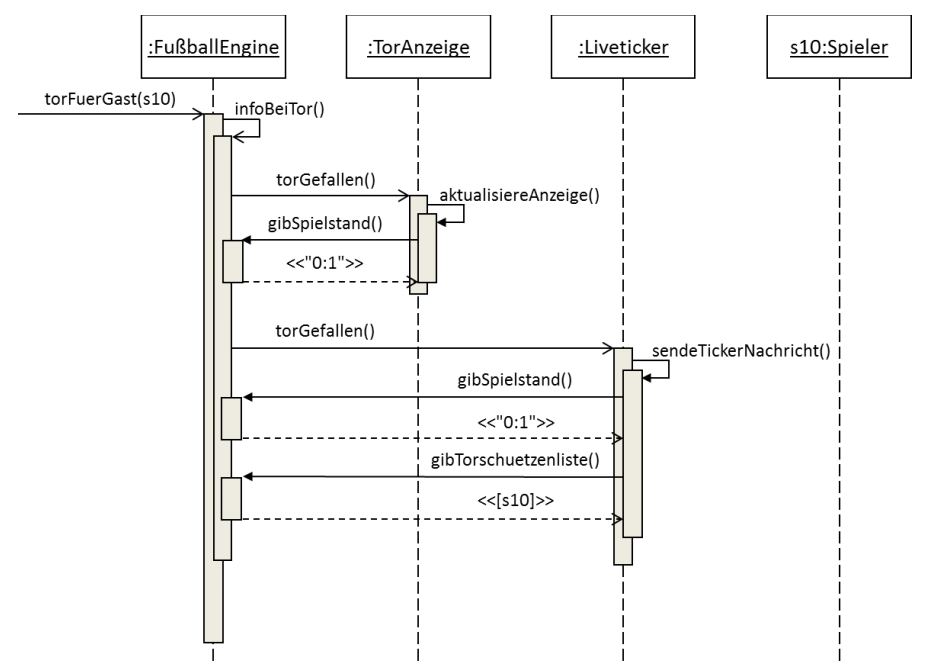
\includegraphics[scale=0.35]{./pics/tut3/obs-task.png}
\end{frame}

\begin{frame}
\frametitle{Musterlösung}
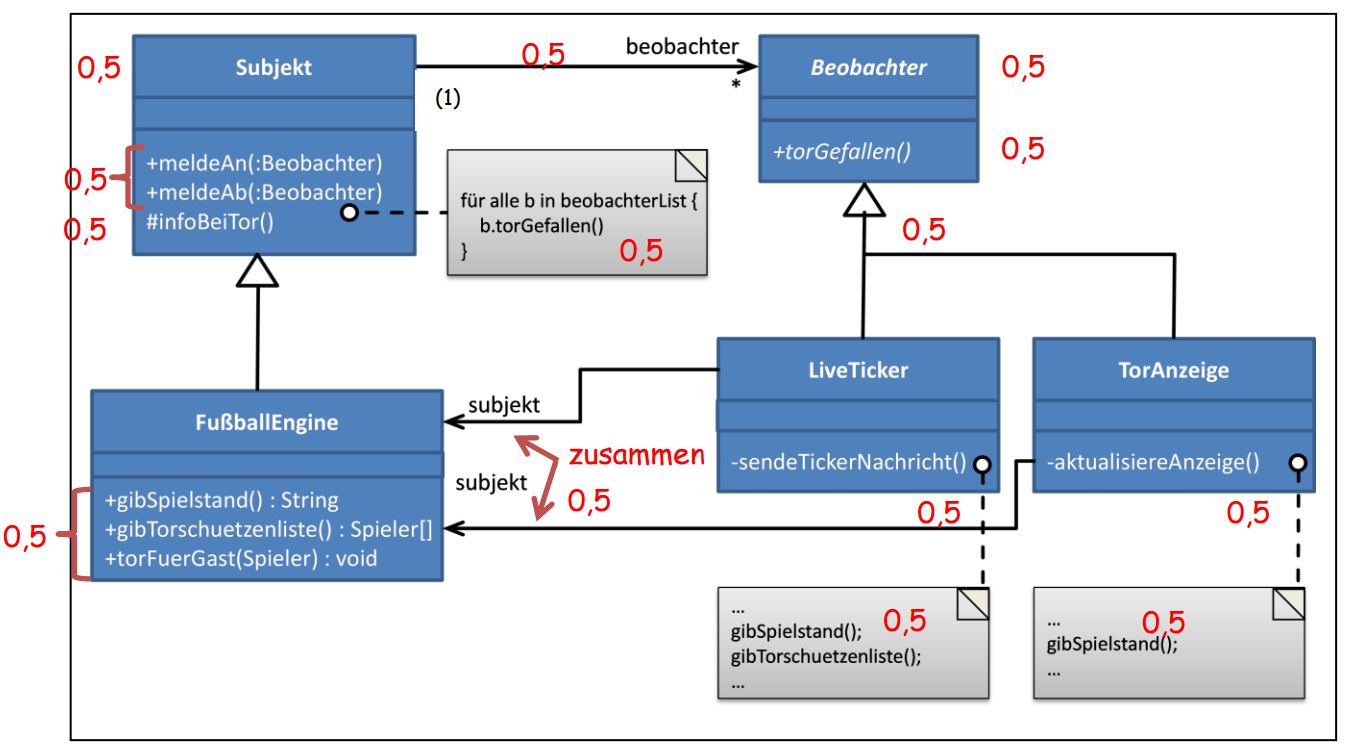
\includegraphics[scale=0.35]{./pics/tut3/obs-task-sol.png}
\end{frame}

	\begin{frame}
		\frametitle{Kategorien der Entwurfsmuster}
		\begin{itemize}
			\item \textbf{Entkopplungs-Muster}
			\begin{itemize}
				\item Adapter \colorbox{green}{fertig}
				\item Beobachter\colorbox{green}{fertig}
				\item Iterator \colorbox{green}{fertig}
				\item Stellvertreter \colorbox{green}{fertig}
				\item Vermittler \colorbox{green}{fertig}
				\item (Brücke)
			\end{itemize}
			\item Varianten-Muster
			\item Zustandshandhabungs-Muster
			\item Steuerungs-Muster
			\item Bequemlichkeits-Muster
		\end{itemize}
	\end{frame}

\section{Gruppenarbeit}
\subsection{Gruppenarbeit}
	\begin{frame}
		\frametitle{Kategorien der Entwurfsmuster}
		\begin{itemize}
			\item Entkopplungs-Muster \colorbox{green}{fertig}
			\item \textbf{Varianten-Muster}
			\begin{itemize}
				\item (Abstrakte Fabrik)
				\item (Besucher)
				\item \textbf{Schablonenmethode}
				\item \textbf{Fabrikmethode}
				\item \textbf{Kompositum}
				\item Strategie \colorbox{green}{fertig}
				\item \textbf{Dekorierer}
			\end{itemize}
			\item Zustandshandhabungs-Muster
			\item Steuerungs-Muster
			\item Bequemlichkeits-Muster
		\end{itemize}
	\end{frame}
	
	\begin{frame}
		\frametitle{Varianten-Muster}
		\begin{block}{Übergeordnetes Ziel}
			\begin{itemize}
				\item Gemeinsamkeiten herausziehen und an einer Stelle beschreiben \pause
				\linebreak $\implies$ keine Wiederholung desselben Codes \pause
				\linebreak $\implies$ bessere Wartbarkeit/Erweiterbarkeit		
			\end{itemize}
		\end{block}
	\end{frame}
	
	\begin{frame}
		\frametitle{Jetzt: Gruppenarbeit}
		\begin{enumerate}
			\item ihr kriegt pro Reihe eine Aufgabe
			\item ihr habt Zeit zum Bearbeiten
			\item Abgleichung mit Musterlösung
			\item ihr stellt den anderen eure Lösung vor
		\end{enumerate}
	\end{frame}

	\begin{frame}
		\frametitle{Vorstellung Dekorierer}
		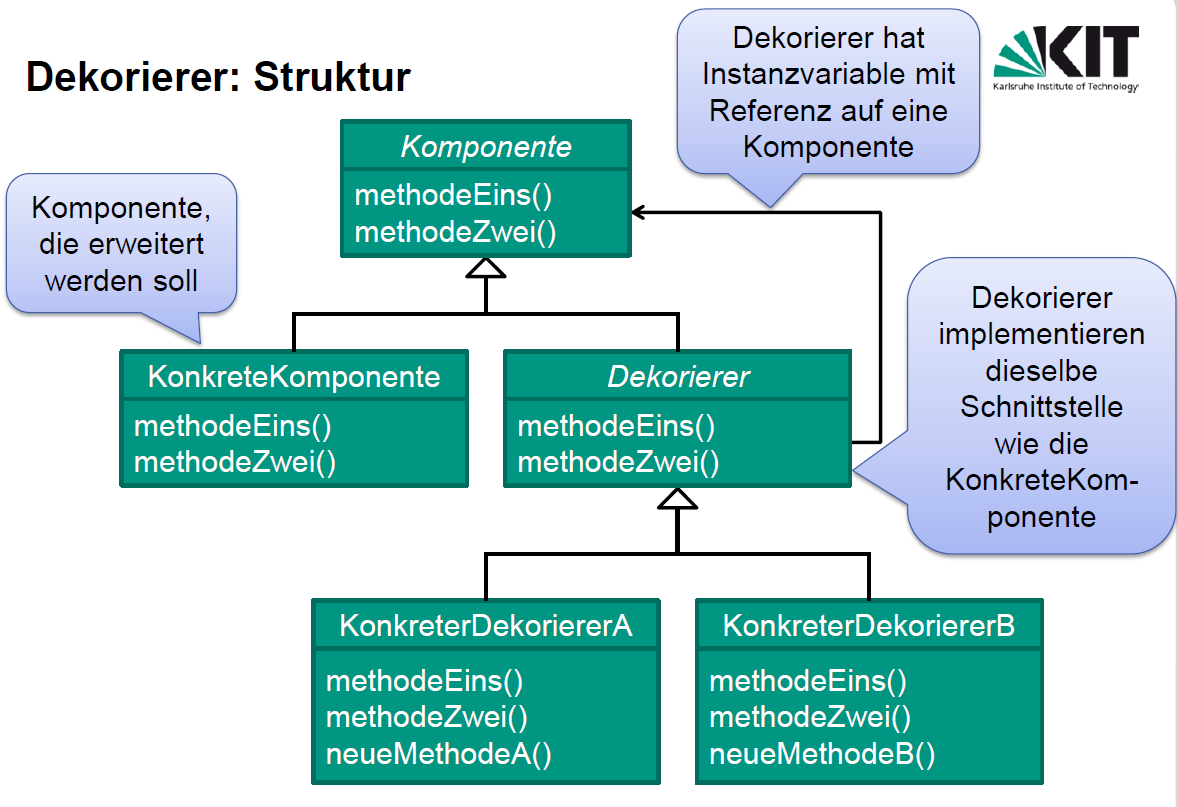
\includegraphics[scale=0.35]{./pics/tut4/decor.png}
	\end{frame}

	\begin{frame}
		\frametitle{MuLö Dekorierer}
		\begin{block}{Wo Gemeinsamkeiten?}
			Die beiden Methoden methodeEins() und methodeZwei().
		\end{block}
		\begin{block}{Wo Variation?}
			In den KonkretenDekorierern bzw. ihren Methoden. Hier: neueMethodeA(), neueMethodeB().
		\end{block}
		\begin{block}{Wozu Instanzvariable?}
			Weiterleitung von Aufrufen der methodeEins() und methodeZwei() an die KonkreteKompenente.
		\end{block}
	\end{frame}

	\begin{frame}
		\frametitle{Vorstellung Kompositum}
		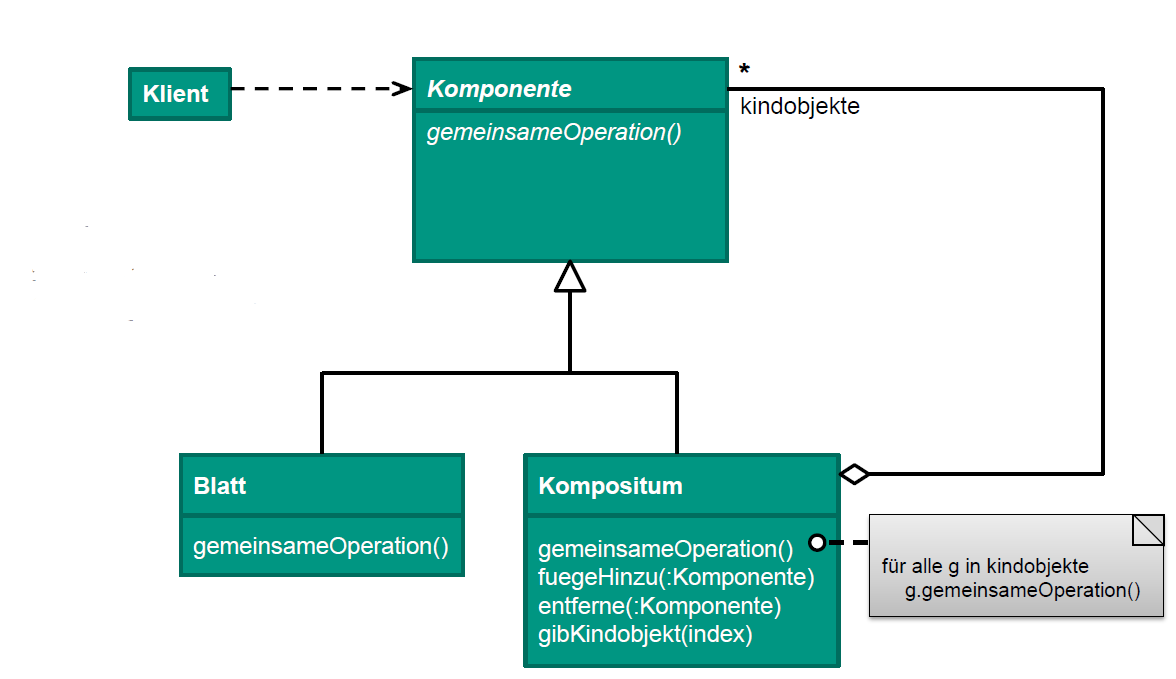
\includegraphics[scale=0.35]{./pics/tut4/comp.png}
	\end{frame}

	\begin{frame}
		\frametitle{MuLö Kompositum}
		\begin{block}{Wo Gemeinsamkeiten?}
			gemeinsameOperation().
		\end{block}
		\begin{block}{Wo Variation?}
			In Blatt/Kompositum-Klassen mit verschiedenen zusätzlichen Operationen.
		\end{block}
		\begin{block}{Zusammengesetzt vs. nicht-zusammengesetzt}
			Kompositum = zusammengesetzt, Blatt = nicht-zusammengesetzt
		\end{block}
	\end{frame}

	\begin{frame}
		\frametitle{Vorstellung Schablonenmethode}
		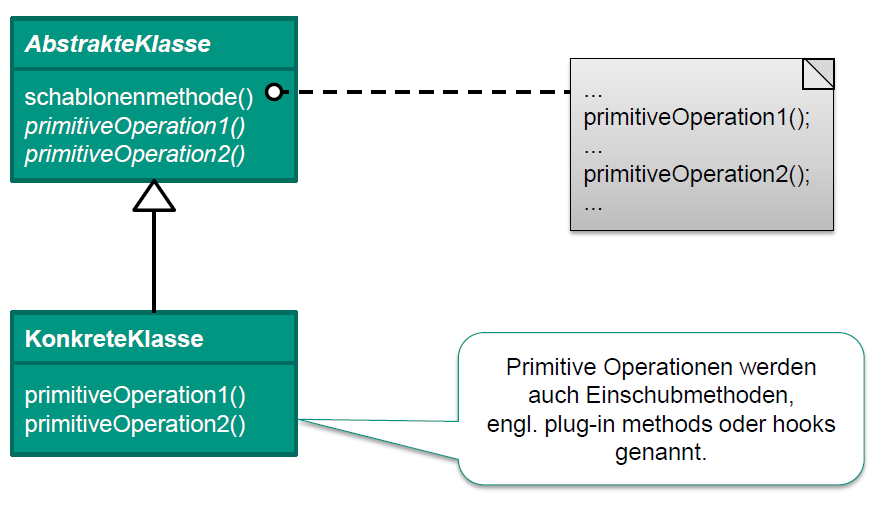
\includegraphics[scale=0.45]{./pics/tut4/schab.png}
	\end{frame}

	\begin{frame}
		\frametitle{MuLö Schablonenmethode}
		\begin{block}{Wo Gemeinsamkeiten?}
			Reihenfolge der Methodenaufrufe in der Schablonenmethode.
		\end{block}
		\begin{block}{Wo Variation?}
			In den Einschubmethoden. (hier: primitiveOperation1() und primitiveOpoeration2())
		\end{block}
		\begin{block}{Schablonenmethode vs. Einschubmethode}
			Einschubmethode ist eine der Methoden, die von der Schablonenmethode aufgerufen wird und deren Implementierung in den Unterklassen stattfindet.
		\end{block}
	\end{frame}

	\begin{frame}
		\frametitle{Vorstellung Fabrikmethode}
		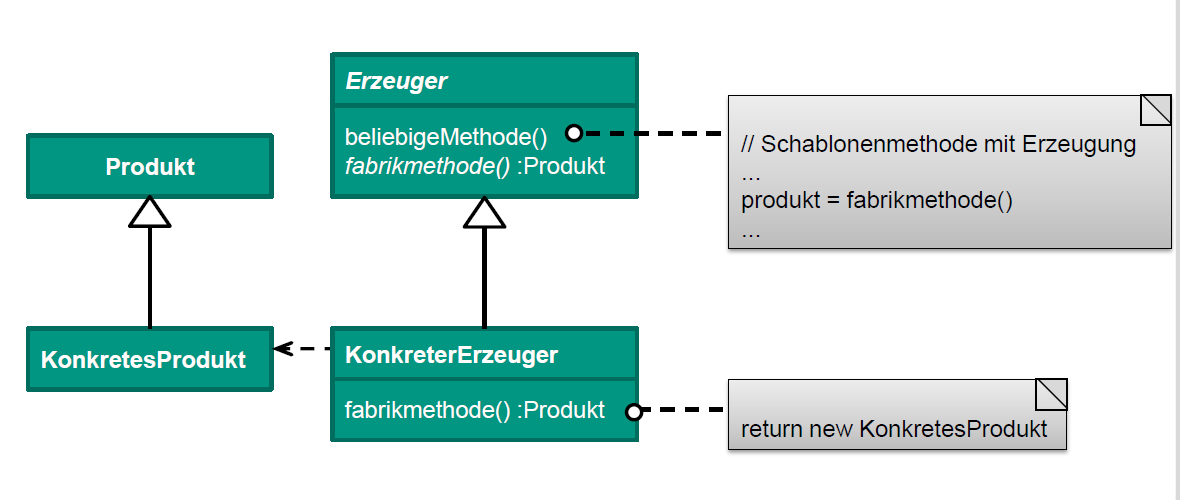
\includegraphics[scale=0.4]{./pics/tut4/fab.png}
	\end{frame}

	\begin{frame}
		\frametitle{MuLö Fabrikmethode}
		\begin{block}{Wo Gemeinsamkeiten?}
			Reihenfolge der Methodenaufrufe in der beliebigenMethode().
		\end{block}
		\begin{block}{Wo Variation?}
			In der Fabrikmethode.
		\end{block}
		\begin{block}{Klasse des Objekts, Oberklasse, Unterklasse}
			Klasse des Objekts = KonkretesProdukt, Oberklasse = Produkt, Unterklasse = KonkreterErzeuger
		\end{block}
		\begin{block}{Unterschied zu Schablonenmethode?}
			Fabrikmethode benutzen, wenn ein Objekt erzeugt wird. Fabrikmethode ist Einschubmethode des Musters "'Schablonenmethode"'.
		\end{block}
		\begin{block}{Wahr/falsch}
			Fabrikmethode ist eine Einschubmethode, keine Schablonenmethode.
		\end{block}
	\end{frame}

	\section{Einzelstück}
	\subsection{Intro}
	\begin{frame}
		\frametitle{Kategorien der Entwurfsmuster}
		\begin{itemize}
			\item Entkopplungs-Muster \colorbox{green}{fertig}
			\item Varianten-Muster \colorbox{green}{fertig}
			\item \textbf{Zustandshandhabungs-Muster}
				\begin{itemize}
					\item \textbf{Einzelstück}
					\item (Fliegengewicht)
					\item \textbf{Memento} 
					\item (Prototyp) 
					\item (Zustand)
				\end{itemize}
			\item Steuerungs-Muster
			\item Bequemlichkeits-Muster
		\end{itemize}
	\end{frame}

	\begin{frame}
		\frametitle{Zustandshandhabungs-Muster}
		\begin{block}{Übergeordnetes Ziel}
			\begin{itemize}
				\item den Zustand eines Objektes beschreiben (wer hätt's gedacht? :D) \pause 
				\item aber unabhängig von dem Zweck des Objekts!
			\end{itemize}
		\end{block}
	\end{frame}

	\begin{frame}
		\frametitle{Einzelstück/Singleton}
		\begin{block}{Problem}
			\begin{itemize}
				\item von einer Klasse soll nur eine Instanz existieren
				\item Konstruktor könnte überall benutzt werden!
			\end{itemize}
		\end{block}
		\pause
		\centering
		\begin{figure}
			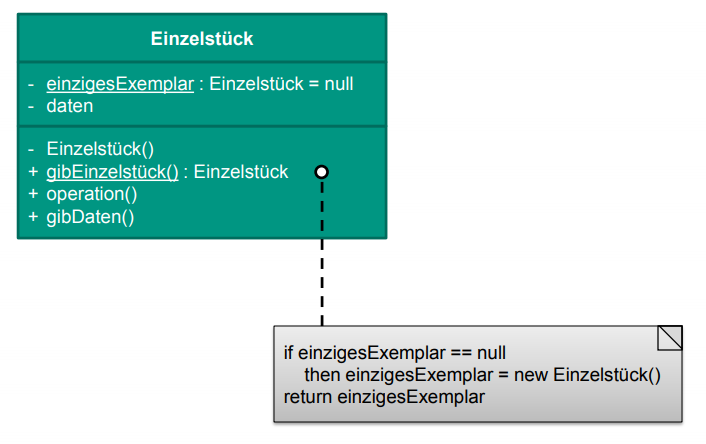
\includegraphics[scale=0.3]{./pics/tut4/singleton.png}
		\end{figure}
		\pause
		Aber warum nicht einfach statisch?\pause ~~ Unterklassenbildung möglich!
	\end{frame}

	\section{Memento}
	\subsection{Memento}
	\begin{frame}
		\frametitle{Memento}
		\begin{block}{Problem}
			\begin{itemize}
				\item internen Zustand eines Objekts "'externalisieren"', um z.B. Zurücksetzen möglich zu machen \pause 
				\item ohne Kapselung zu verletzten!
			\end{itemize}
		\end{block}
		\pause
		\centering
		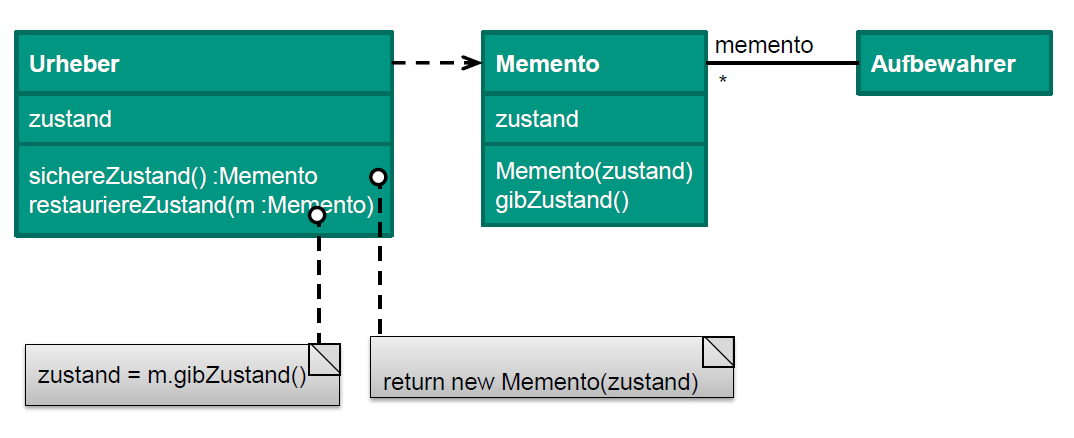
\includegraphics[scale=0.4]{./pics/tut4/mem.png}
	\end{frame}

	\begin{frame}
		\frametitle{Memento}
		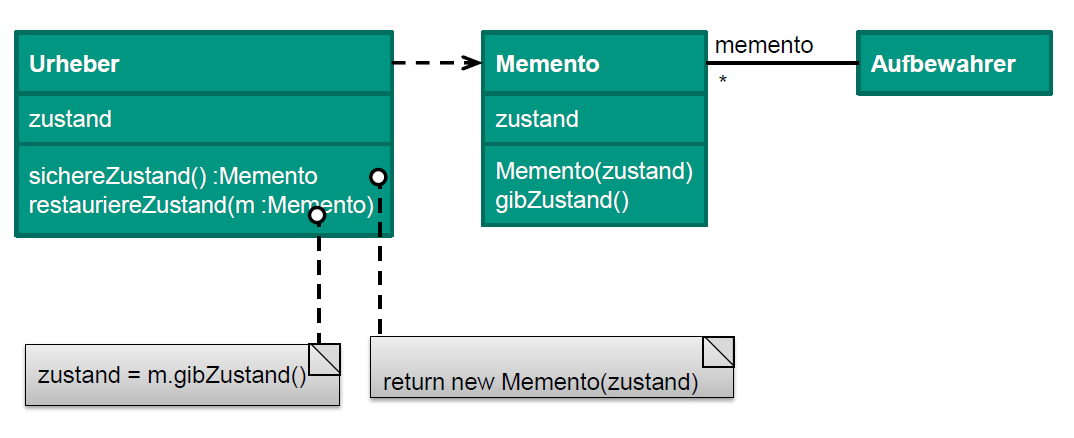
\includegraphics[scale=0.4]{./pics/tut4/mem.png}
		\begin{block}{Problem gelöst?}
			\begin{itemize}
				\pause
				\item Ja
				\begin{itemize}
					\pause
					\item Zustand durch Memento externalisiert \pause
					\item Kapselung nicht verletzt (Nutzer ruft nur sichereZustand() auf und kriegt neuen Memento)
				\end{itemize}
			\end{itemize}
		\end{block}
\end{frame}

\section{Befehl}
	\subsection{Intro}
	\begin{frame}
		\frametitle{Kategorien der Entwurfsmuster}
		\begin{itemize}
			\item Entkopplungs-Muster \colorbox{green}{fertig}
			\item Varianten-Muster \colorbox{green}{fertig}
			\item Zustandshandhabungs-Muster \colorbox{green}{fertig}
			\item \textbf{Steuerungs-Muster} 
				\begin{itemize}
					\item \textbf{Befehl}
					\item (master/worker)
				\end{itemize}
			\item Bequemlichkeits-Muster
		\end{itemize}
	\end{frame}
	
	\begin{frame}
		\frametitle{Steuerungs-Muster}
		\begin{block}{Übergeordnetes Ziel}
			\begin{itemize}
				\item steuern den Kontrollfluss \pause 
				\linebreak $\implies$ zur richtigen Zeit richtige Methoden aufrufen
			\end{itemize}
		\end{block}
	\end{frame}

	\begin{frame}
		\frametitle{Befehl}
		\begin{block}{Problem}
			\begin{itemize}
				\item Parametrisieren von Objekten mit einer auszuführenden Aktion \pause 
				\item komplexe Operationen aus primitiven Operationen aufbauen \pause
				\linebreak $\implies$ Befehl nicht als Methode, sondern als Objekt modellieren
			\end{itemize}
		\end{block}
		\pause
		\centering
		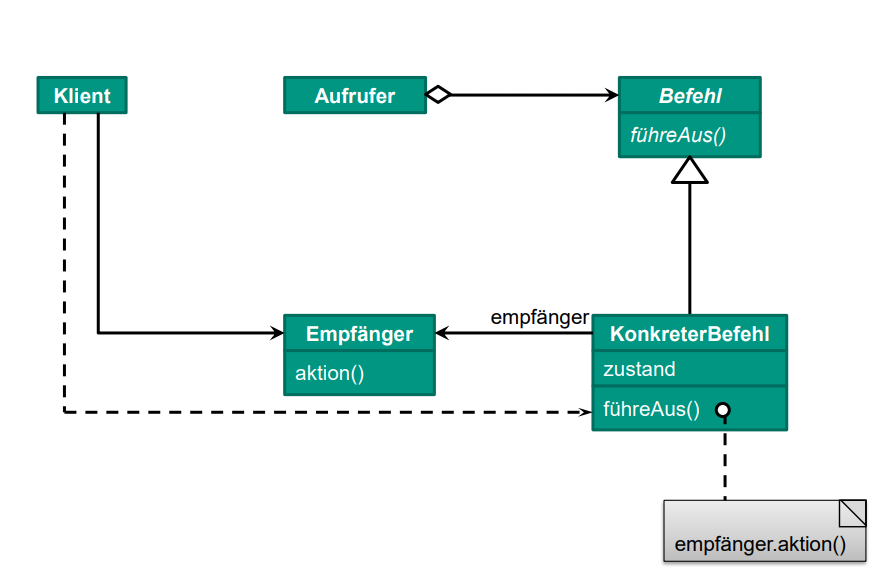
\includegraphics[scale=0.35]{./pics/tut4/command.png}
	\end{frame}

	\begin{frame}
		\frametitle{Befehl}
		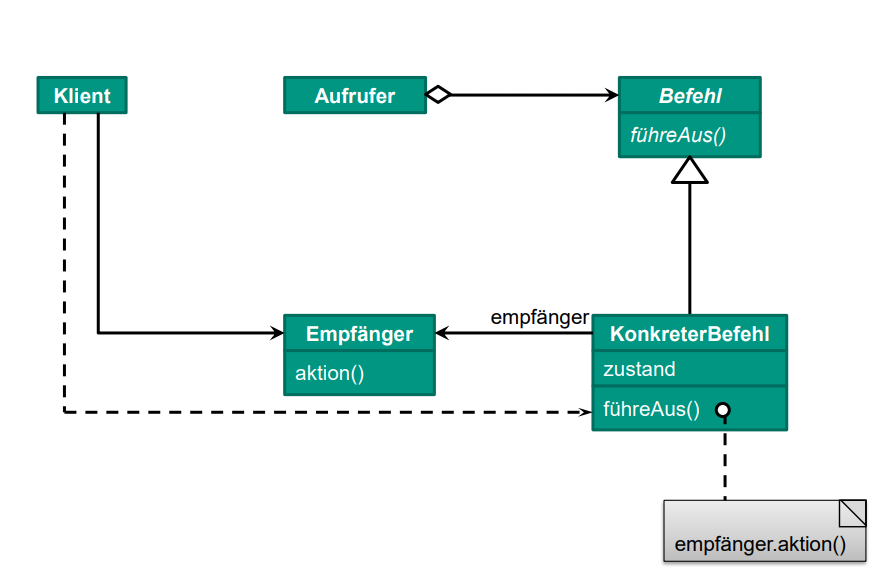
\includegraphics[scale=0.35]{./pics/tut4/command.png}
		\begin{block}{Was haben wir erreicht?}
			\begin{itemize}
				 \pause
				\item Austauschbarkeit: Befehle unabhängig vom Aufrufer, universell einsetzbar
			\end{itemize}
		\end{block}
	\end{frame}
	
	\begin{frame}
		\frametitle{Befehl}
		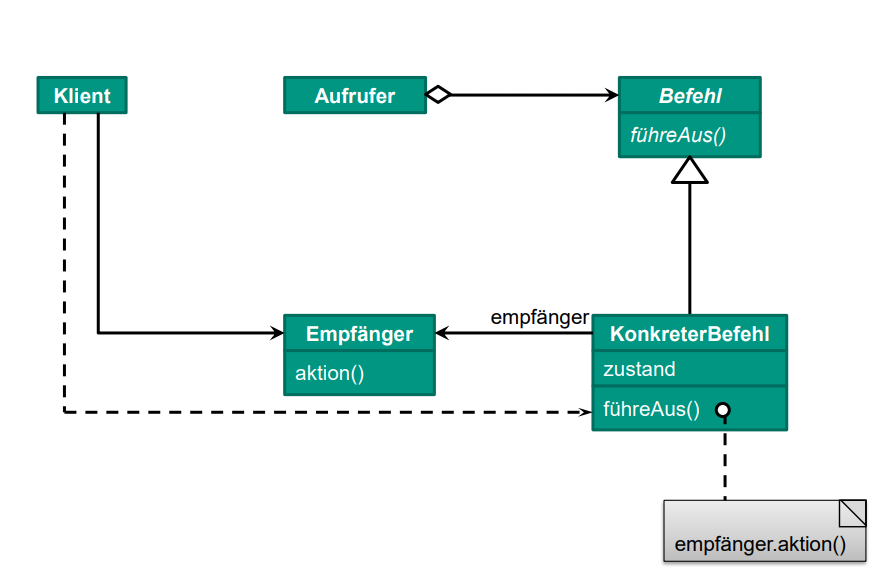
\includegraphics[scale=0.4]{./pics/tut4/command.png}
		\linebreak
		\centering \large Beispiel!
	\end{frame}
	
	\begin{frame}
		\frametitle{Quiz (Ankreuzaufgaben aus Klausuren)}
		Wahr oder falsch?
		\begin{itemize}
			\item Bei dem Entwurfsmuster Befehl kennt der Empfänger den Befehl nicht, jedoch der Befehl den Empfänger. \pause \colorbox{green}{wahr} \pause
			\item Ein Aufbewahrer im Entwurfsmuster Memento kann beliebig viele Mementos verwalten. Für die Restauration im Falle eines Reset ist er allerdings nicht verantwortlich. \pause \colorbox{green}{wahr} \pause
			\item Die Fabrikmethode sorgt dafür, dass nur eine einzige Instanz einer Klasse fabriziert wird. \pause \colorbox{red}{falsch} \pause 
			\item Eine Schablonenmethode ist immer auch eine Fabrikmethode. \pause \colorbox{red}{falsch} \pause
			\item Eine Komponente kann immer nur mit einem einzigen Dekorierer versehen werden. \pause \colorbox{red}{falsch}
		\end{itemize}
	\end{frame}
	
	
	\begin{frame}
		\frametitle{Für die Klausur}
		\begin{itemize}
			\item Entwurfsmuster kommen sehr sehr sehr wahrscheinlich dran! \pause 
			\item Kategorien helfen beim Lernen \pause
			\item jedes Entwurfsmuster erfüllt einen bestimmten Zweck 
			\linebreak $\implies$ nicht nur die Klassen und Methoden auswendig lernen, sondern das Prinzip verstehen \pause
			\item bei Unklarheiten in Head First Design Patterns nachlesen ;)
		\end{itemize}
	\end{frame}
	
\section{Tipps}
	\subsection{Tipps}
	\begin{frame}
		\frametitle{Tipps - 5. Übungsblatt}
			\begin{exampleblock}{Aufgabe 1: Shutterpile: Refaktorisierung + Entwurfsmuster anwenden} 
				\begin{itemize}
					\item Entwurfsmuster anschauen
					\item alte Tests verwenden + evtl. neue schreiben
				\end{itemize}
			\end{exampleblock}
			\pause
			\begin{exampleblock}{Aufgabe 2: cmd-Programm für Pipeline} 
				\begin{itemize}
					\item wie Shutterpile-cmd, nur kommen nach Parameter \enquote{-p} noch Werte
					\item \url{https://commons.apache.org/proper/commons-cli/usage.html}
				\end{itemize}
			\end{exampleblock}
	\end{frame}

	\begin{frame}
		\frametitle{Tipps - 5. Übungsblatt}
			\begin{exampleblock}{Aufgabe 3: Wo sind Entwurfsmuster in Shutterpile?}
				\begin{itemize}
					\item Maßstab ist Musterlösung
					\item nur finden reicht nicht, auch erklären wie und warum
				\end{itemize}
			\end{exampleblock}
			\pause
			\begin{exampleblock}{Aufgabe 4: Entwurfsmuster in Java-API}
				\begin{itemize}
					\item es handelt sich um \enquote{einfachere} Muster
				\end{itemize}
			\end{exampleblock}
			\pause
			\begin{exampleblock}{Aufgabe 5: Entwurfsmuster - Kaffeemaschine}
				\begin{itemize}
					\item ein Muster anwenden
				\end{itemize}
			\end{exampleblock}
	\end{frame}
	
	\subsection{Abgabe}
	\begin{frame}
		\frametitle{Denkt dran!}
		\begin{alertblock}{Abgabe}
			\begin{itemize}
				\item Deadline am 27.6. um 12:00
				\item Aufgabe 3-5 handschriftlich
			\end{itemize}
		\end{alertblock}
	\end{frame}
		
	\begin{frame}
		\frametitle{Bis dann! (dann  := 03.07.18)}
		\centering
		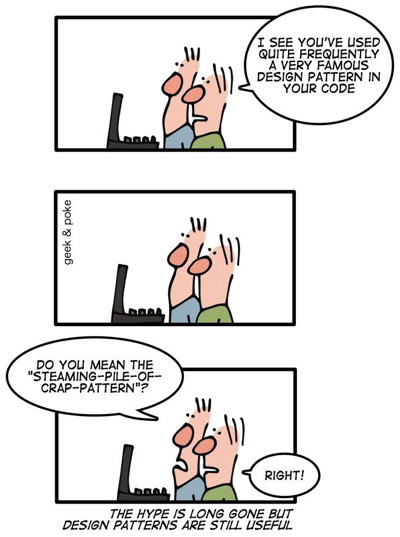
\includegraphics[scale=0.4]{./comics/patterns.jpg}
	\end{frame}

\end{document}